% Chapter 2

\chapter{Methodology} % Main chapter title

\label{Chapter2} % For referencing the chapter elsewhere, use \ref{Chapter1} 

\lhead{2. \emph{Methodology}} % This is for the header on each page - perhaps a shortened title 


Given the epicentral intensity ($I_0$) a set of observation of macroseismic intensity is  first divided into bins  of distance. Then it is assumed that the attenuation behavior in these bins is homogeneous and can be described by the following binomial distribution:


\begin{equation}
P(I_s = i\mid I_0 = i_0, p) = \binom{i_0}{i} p^i(1-p)^{i_0-i}
\label{eqn:likelihood1}
\end{equation}


Since the governing parameter p is also unknown it is treated, according to the Bayesian paradigm, as a random variable and a Beta distribution is defined.
\begin{equation}
P(p) = \dfrac{1}{B(\alpha,\beta)} p^{\alpha-1} (1-p)^{\beta -1} 
\label{eqn:prior}
\end{equation}

This means that for each distance bin a Bayesian model with a likelihood of a binomial distribution and a prior of a Beta distribution is constructed and subsequently the observations for each distance bin are used to estimate the p parameter.

\begin{subequations}
\begin{align}
P(p \mid I_s) & = \dfrac{P(I_s \mid p)}{P(I_s)} P(p) \\
 & \propto p^i(1-p)^{i_0-i} * p^{\alpha-1} (1-p)^{\beta -1}\\
 & \propto p^{\alpha + i -1}(1-p)^{\beta +i_0-i -1}\\
 & \propto p^{\alpha' -1}(1-p)^{\beta' -1}
\end{align}
\label{eqn:posterior}
\end{subequations}

Choosing a Beta distribution as prior has the advantage of a conjugate model, so the calculations are performed more easily because the posterior distribution is again a beta distribution. To compute the posterior distribution $P(p \mid I_s)$ only the parameters $\alpha$  and $\beta$ have to be updated:
\begin{equation}
\alpha' = \alpha + \sum^N_{n= 1} i_s \hspace{2cm} \beta' =  \beta + \sum^N_{n= 1} (I_0 - i_s)
\label{eqn:updatehyper}
\end{equation}

Because the distance is discretized it is just possible to calculate the probability distribution for each distance bin. To overcome this obstacle and to have a continuous model the mode for each distance bin is used to construct a smoothing function using an inverse power function.

\begin{equation}
g(d) =  \left(\dfrac{\gamma_1}{\gamma_1 + d}\right)^{\gamma_2}
\label{eqn:smoothing}
\end{equation}

The smoothing function is subsequently applied to the mean of the posterior distribution $\hat{p}$:

\begin{equation}
\hat{p} = E\left[P(p \mid I_s)\right] = \dfrac{\alpha'}{\alpha' + \beta'}
\label{eqn:update}
\end{equation}

In order to forecast macroseismic intensities at any given distance the fitted smoothing function g(d) is used as an estimate of the p parameter and plugged in to the binomial distribution:


\begin{equation}
P(I_s = i\mid I_0, g(d)) = \binom{I_0}{i} g(d)^i(1-g(d))^{i_0-i}
\label{eqn:forecast}
\end{equation}

This approach has some special properties and assumption. Since the binomial distribution is a discrete probability distribution the categorical nature of intensities is respected. In contrast to a multinomial-Dirichlet model it has the advantage of needing only two parameters ($\alpha$ and $\beta$) to be estimated. Because the binomial distribution approaches the Gaussian distribution in the limits it has also a kind of neighboring effect, meaning that intensities next to the intensity with highest probability are assigned the next lowest probability. This models actually some reasonable physical behavior because for example in a scenario were the highest probability is given to intensity VII it wouldn't be logical that the second highest probability would be intensity II. At this point the model assumes that the earthquake process is linked to a point source, e.g. the isoseismals are circles.\\

\begin{figure}[!htpb]
 \centering
		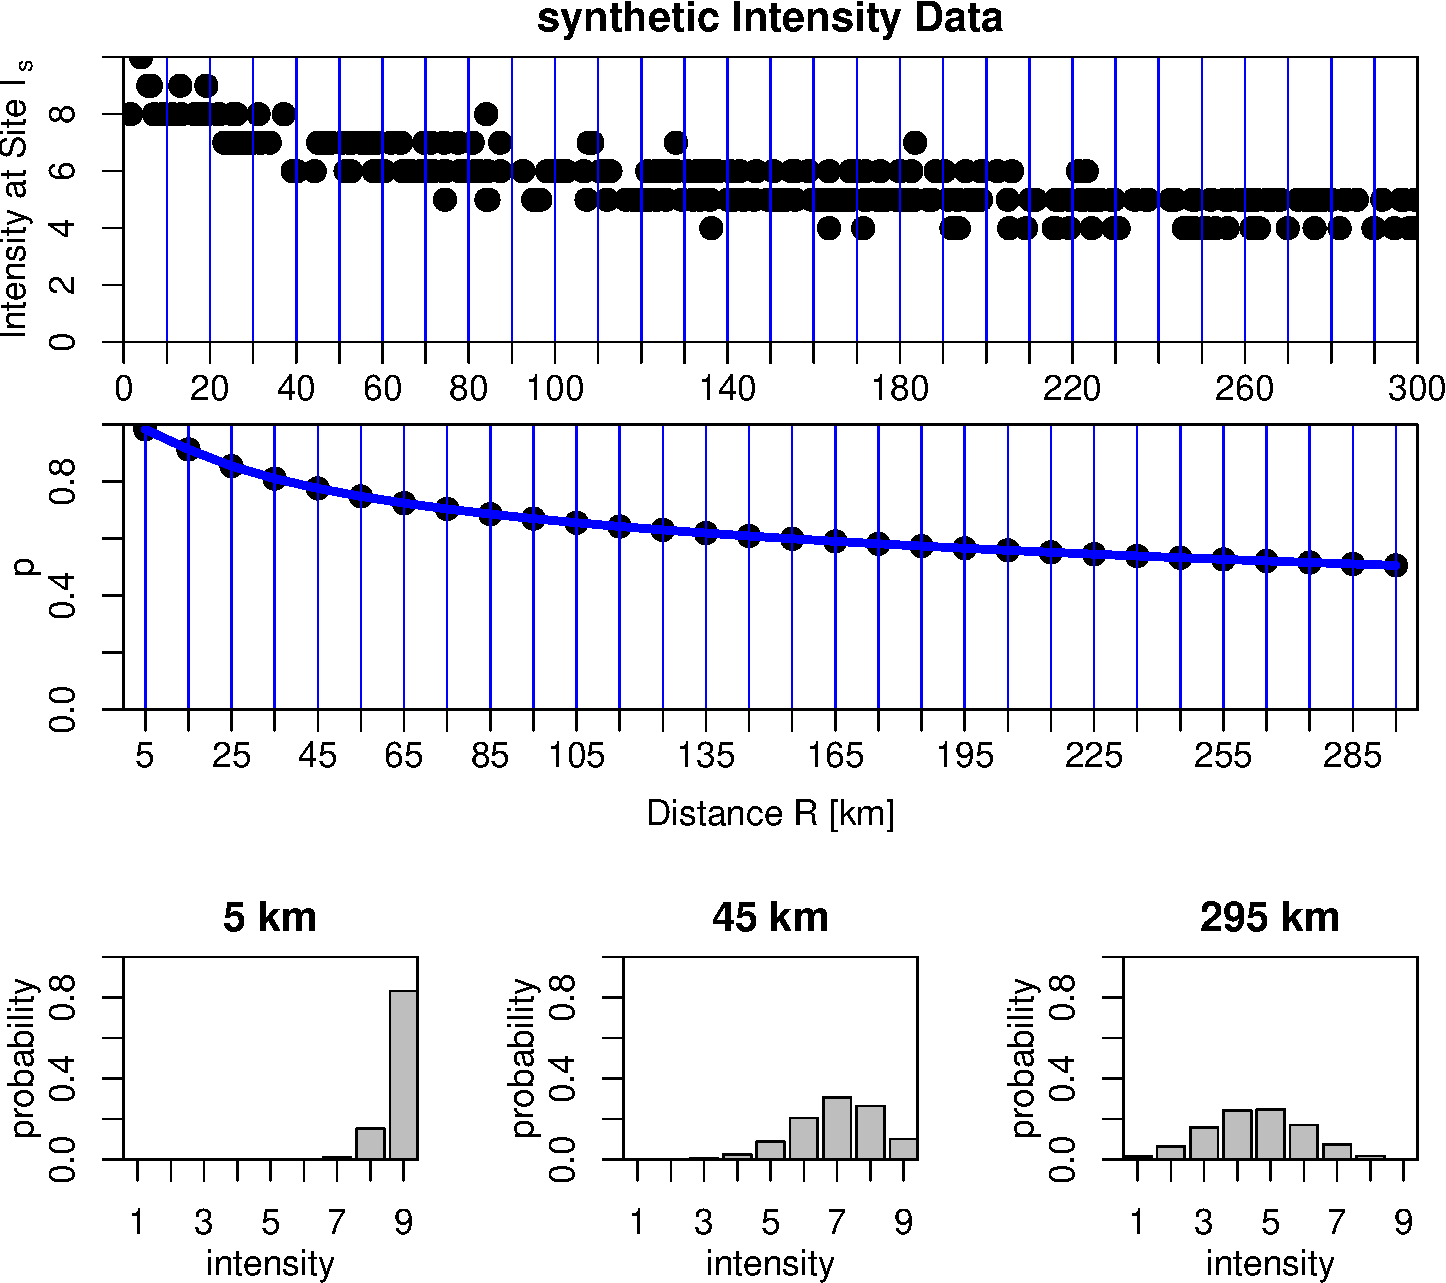
\includegraphics[scale=0.6]{Figures/example.pdf}
		\rule{35em}{0.5pt}
	\caption[Example]{Example of the process of developing groundmotion models. The top figure shows a data set of macroseismic observations. These are discretized into distance bins with a width of 10 km. In each distance bin the abservations are used to update the prior parameter of the Beta distribution. In the middle figure the mean of the posterior Beta distributions is assigned to the middle of the distance bins a smoothing function is used to get values of the p parameter for every distance. The bottom figure shows the probability distribution for different distances once the posterior mean of the Beta distribution is supplied to the binomial distribution.}
	\label{fig:example}
\end{figure}

